\section{Example Using Two Tetrahedra}
\label{sec:example:twotet4}

PyLith features discussed in this example:
\begin{itemize}
\item Quasi-static solution
\item Mesh ASCII format
\item Dirichlet boundary conditions
\item Kinematic fault interface conditions
\item Linearly elastic isotropic material
\item VTK output
\item Linear tetrahedral cells
\item SimpleDB spatial database
\item ZeroDispDB spatial database
\end{itemize}
All of the files necessary to run the examples are contained in the
directory \filename{examples/twocells/twotet4.}


\subsection{Overview}

This example is a simple 3D example of a quasi-static finite element
problem. It is a mesh composed of two linear tetrahedra subject to
displacement boundary conditions, and is probably the simplest example
of a 3D elastic problem. Due to the simple geometry of the problem,
the mesh may be constructed by hand, using PyLith mesh ASCII format.
In this example, we will walk through the steps necessary to
construct, run, and view two problems that use the same mesh. In
addition to this manual, each of the files for the example problem
includes extensive comments.


\subsection{Mesh Description}

The mesh consists of two tetrahedra forming a pyramid shape (Figure
\vref{fig:twotet4-mesh}). The mesh geometry and topology is described
in the file \filename{twotet4.mesh}, which is in PyLith mesh ASCII
format.

\begin{figure}
  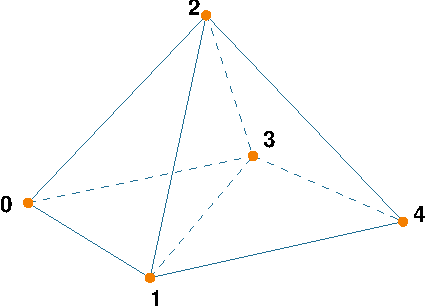
\includegraphics{examples/figs/twotet4-mesh}
  \caption{Mesh composed of two linear tetrahedral cells used for example problems.}
  \label{fig:twotet4-mesh}
\end{figure}


\subsection{Additional Common Information}

In addition to the mesh, the two example problems share additional
information, which we place in \filename{pylithapp.cfg}.


\subsection{Axial Displacement Example}

The first example problem is extension of the mesh along the diagonal,
extending along the base of the pyramid between two opposing vertices.
Parameter settings that override or augment those in \filename{pylithapp.cfg}
are contained in the file \filename{axialdisp.cfg}. These settings include:
\begin{inventory}
  \facilityitem{pylithapp.timedependent.bc.bc}{Defines which degrees of freedom
    are being constrained (\texttt{x}, \texttt{y}, and \texttt{z}), gives
    the label (defined in \filename{twotet4.mesh}) defining the points desired,
    assigns a label to the boundary condition set, and gives the name
    of the spatial database defining the boundary conditions (\filename{axialdisp.spatialdb}).}
\end{inventory}
The values for the Dirichlet boundary conditions are described in
the file \filename{axialdisp.spatialdb}, as specified in \filename{axialdisp.cfg}.
Because data are being specified using two control points (rather
than being uniform over the mesh), the data dimension is one.

The files containing common information (\filename{twotet4.mesh},
\filename{pylithapp.cfg}, \filename{matprops.spatialdb}) along with
the problem-specific files (\filename{axialdisp.cfg},
\filename{axialdisp.spatialdb}) provide a complete description of the
problem, and we can then run this example by typing
\begin{shell}
$ pylith axialdisp.cfg
\end{shell}
If the problem ran correctly, you should be able to produce a figure
such as Figure \vref{fig:twotet4-axial}, which was generated using
ParaView.

\begin{figure}
  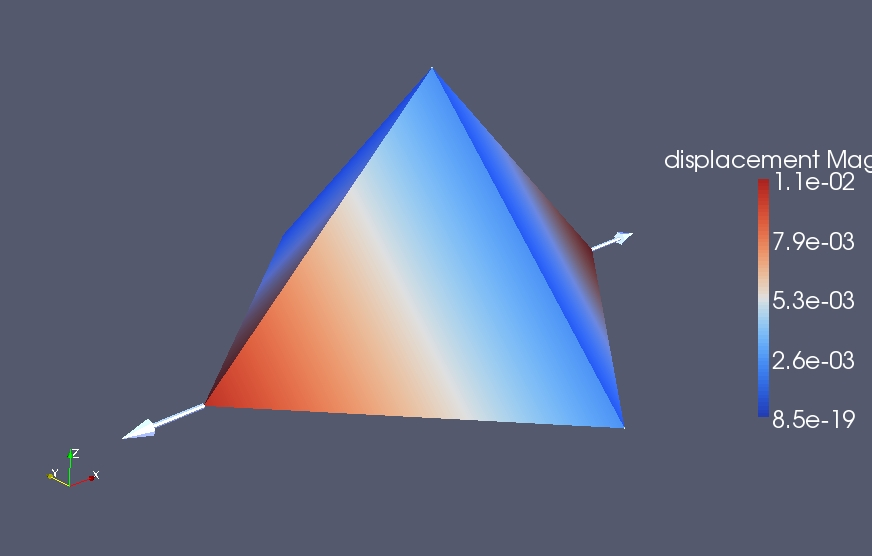
\includegraphics[scale=0.33]{examples/figs/twotet4-axialdisp}
  \caption{Color contours and vectors of displacement for the axial displacement
    example using a mesh composed of two linear tetrahedral cells.}
  \label{fig:twotet4-axial}
\end{figure}


\subsection{Kinematic Fault Slip Example}

The next example problem is a left-lateral fault slip applied between
the two tetrahedral cells using kinematic cohesive cells. The vertices
away from the fault are held fixed in the \texttt{x}, \texttt{y},
and \texttt{z} directions. Parameter settings that override or augment
those in \filename{pylithapp.cfg} are contained in the file \filename{dislocation.cfg}.
These settings include:
\begin{inventory}
  \facilityitem{pylithapp.timedependent.bc.bc}{Defines which degrees of freedom
    are being constrained (\texttt{x}, \texttt{y}, and \texttt{z}), gives
    the label (defined in \filename{twotet4.mesh}) defining the points desired,
    and assigns a label to the boundary condition set. Rather than specifying
    a spatial database file to define the boundary conditions, we use
    the default spatial database (ZeroDispDB) for the Dirichlet boundary
    condition, which sets the displacements to zero.}
  \facilityitem{pylithapp.timedependent.interfaces}{Gives the label (defined in
    \filename{twotet4.mesh}) defining the points on the fault, provides
    quadrature information, and then gives database names for material
    properties (needed for conditioning), fault slip, peak fault slip
    rate, and fault slip time.}
\end{inventory}
The fault example requires three additional database files that were
not needed for the simple displacement examples. The first file
(\filename{dislocation\_slip.spatialdb}) specifies 0.01 m of
left-lateral fault slip for the entire fault.  The data dimension is
zero since the same data are applied to all points in the set. The
default slip time function is a step-function, so we also must provide
the time at which slip begins. The elastic solution is associated with
advancing from $t=-dt$ to $t=0$, so we set the slip initiation time
for the step-function to 0 in
\filename{dislocation\_sliptime.spatialdb}.

The files containing common information (\filename{twotet4.mesh}, \filename{pylithapp.cfg},
\filename{matprops.spatialdb}) along with the problem-specific files
(\filename{dislocation.cfg, dislocation\_slip.spatialdb},
\filename{dislocation\_sliptime.spatialdb}) provide a complete description
of the problem, and we can then run this example by typing
\begin{shell}
$ pylith dislocation.cfg
\end{shell}
If the problem ran correctly, you should be able to generate a figure
such as Figure \vref{fig:twotet4-disloc}, which was generated using
ParaView.

\begin{figure}
  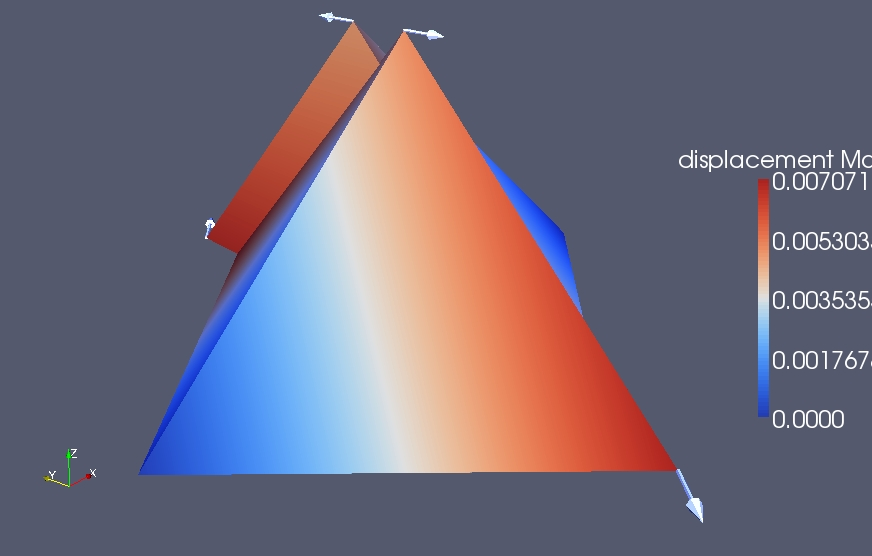
\includegraphics[scale=0.33]{examples/figs/twotet4-dislocation}
  \caption{Color contours and vectors of displacement for the kinematic fault
    example using a mesh composed of two linear tetrahedral cells.}
  \label{fig:twotet4-disloc}
\end{figure}


% End of file
